\documentclass[tikz,border=8pt]{standalone}
% Shared look for every TikZ diagram. Load with \input{../../tools/tikz-style.tex}
\usepackage[T1]{fontenc}
\usepackage{lmodern}
\renewcommand{\sfdefault}{lmr}  % diagrams use the same serif as the text
\usetikzlibrary{arrows.meta, positioning, shapes.geometric, calc, fit, backgrounds}
\definecolor{cblue}{HTML}{4C78A8}
\definecolor{corange}{HTML}{F58518}
\definecolor{cgreen}{HTML}{54A24B}
\definecolor{cred}{HTML}{E45756}
\definecolor{cpurple}{HTML}{B279A2}
\definecolor{cgrey}{HTML}{6B6B6B}
\tikzset{
  every picture/.style={font=\sffamily, line width=1.2pt},
  box/.style={draw=#1, fill=#1!12, rounded corners=4pt, align=center, inner sep=7pt, minimum height=1.1cm},
  box/.default=cgrey,
  arrow/.style={-{Stealth[length=3mm]}, draw=cgrey, line width=1.4pt},
  title/.style={font=\sffamily\bfseries\Large},
  note/.style={font=\sffamily\small, text=cgrey, align=center},
}
\AtBeginDocument{\hyphenpenalty=10000 \exhyphenpenalty=10000}

\begin{document}
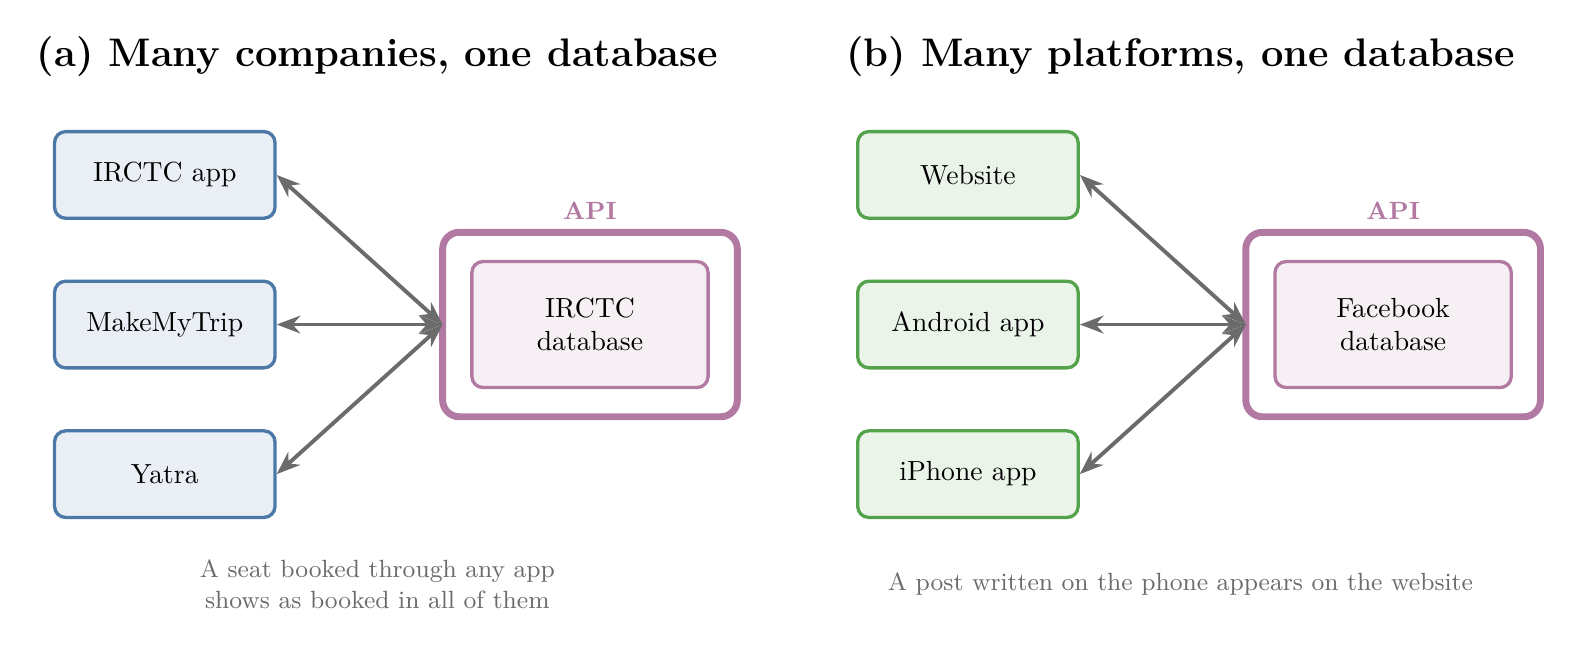
\begin{tikzpicture}
  % (a) many companies, one database
  \node[box=cpurple, minimum width=3.0cm, minimum height=1.6cm] (db1) at (0,0) {IRCTC\\database};
  \draw[draw=cpurple, line width=2.5pt, rounded corners=6pt] ($(db1.south west)+(-0.35,-0.35)$) rectangle ($(db1.north east)+(0.35,0.35)$);
  \node[font=\sffamily\small\bfseries, text=cpurple] at ($(db1.north)+(0,0.62)$) {API};
  \foreach \name/\y/\i in {IRCTC app/1.9/1, MakeMyTrip/0/2, Yatra/-1.9/3} {
    \node[box=cblue, minimum width=2.8cm] (c\i) at (-5.4,\y) {\name};
    \draw[{Stealth[length=3mm]}-{Stealth[length=3mm]}, draw=cgrey, line width=1.4pt] (c\i.east) -- ($(db1.west)+(-0.35,0)$);
  }
  \node[title] at (-2.7,3.4) {(a) Many companies, one database};
  \node[note, text width=7.5cm] at (-2.7,-3.3) {A seat booked through any app shows as booked in all of them};
  % (b) many platforms, one database
  \begin{scope}[xshift=10.2cm]
  \node[box=cpurple, minimum width=3.0cm, minimum height=1.6cm] (db2) at (0,0) {Facebook\\database};
  \draw[draw=cpurple, line width=2.5pt, rounded corners=6pt] ($(db2.south west)+(-0.35,-0.35)$) rectangle ($(db2.north east)+(0.35,0.35)$);
  \node[font=\sffamily\small\bfseries, text=cpurple] at ($(db2.north)+(0,0.62)$) {API};
  \foreach \name/\y/\i in {Website/1.9/1, Android app/0/2, iPhone app/-1.9/3} {
    \node[box=cgreen, minimum width=2.8cm] (d\i) at (-5.4,\y) {\name};
    \draw[{Stealth[length=3mm]}-{Stealth[length=3mm]}, draw=cgrey, line width=1.4pt] (d\i.east) -- ($(db2.west)+(-0.35,0)$);
  }
  \node[title] at (-2.7,3.4) {(b) Many platforms, one database};
  \node[note, text width=7.5cm] at (-2.7,-3.3) {A post written on the phone appears on the website};
  \end{scope}
\end{tikzpicture}
\end{document}
